 %Version 3.1 December 2024
  % See section 11 of the User Manual for version history
  %
  %%%%%%%%%%%%%%%%%%%%%%%%%%%%%%%%%%%%%%%%%%%%%%%%%%%%%%%%%%%%%%%%%%%%%%
  %%                                                                 %%
  %% Please do not use \input{...} to include other tex files.       %%
  %% Submit your LaTeX manuscript as one .tex document.              %%
  %%                                                                 %%
  %% All additional figures and files should be attached             %%
  %% separately and not embedded in the \TeX\ document itself.       %%
  %%                                                                 %%
  %%%%%%%%%%%%%%%%%%%%%%%%%%%%%%%%%%%%%%%%%%%%%%%%%%%%%%%%%%%%%%%%%%%%%

  %%\documentclass[referee,sn-basic]{sn-jnl}% referee option is meant for double line spacing

  %%=======================================================%%
  %% to print line numbers in the margin use lineno option %%
  %%=======================================================%%

  %%\documentclass[lineno,pdflatex,sn-basic]{sn-jnl}% Basic Springer Nature Reference Style/Chemistry Reference Style

  %%=========================================================================================%%
  %% the documentclass is set to pdflatex as default. You can delete it if not appropriate.  %%
  %%=========================================================================================%%

  %%\documentclass[sn-basic]{sn-jnl}% Basic Springer Nature Reference Style/Chemistry Reference Style

  %%Note: the following reference styles support Namedate and Numbered referencing. By default the style follows the most common
  %%style. To switch between the options you can add or remove “Numbered” in the optional parenthesis.
  %%The option is available for: sn-basic.bst, sn-chicago.bst%

  %%\documentclass[pdflatex,sn-nature]{sn-jnl}% Style for submissions to Nature Portfolio journals
  \documentclass[pdflatex,sn-basic]{sn-jnl}% Basic Springer Nature Reference Style/Chemistry Reference Style
  %%\documentclass[pdflatex,sn-mathphys-num]{sn-jnl}% Math and Physical Sciences Numbered Reference Style
  %%\documentclass[pdflatex,sn-mathphys-ay]{sn-jnl}% Math and Physical Sciences Author Year Reference Style
  %%\documentclass[pdflatex,sn-aps]{sn-jnl}% American Physical Society (APS) Reference Style
  %%\documentclass[pdflatex,sn-vancouver-num]{sn-jnl}% Vancouver Numbered Reference Style
  %%\documentclass[pdflatex,sn-vancouver-ay]{sn-jnl}% Vancouver Author Year Reference Style
  %%\documentclass[pdflatex,sn-apa]{sn-jnl}% APA Reference Style
  %%\documentclass[pdflatex,sn-chicago]{sn-jnl}% Chicago-based Humanities Reference Style

  %%%% Standard Packages
  %%<additional latex packages if required can be included here>

  \usepackage{graphicx}%
  \usepackage{multirow}%
  \usepackage{amsmath,amssymb,amsfonts}%
  \usepackage{amsthm}%
  \usepackage{mathrsfs}%
  \usepackage[title]{appendix}%

  \usepackage{xcolor}%
  \usepackage{textcomp}%
  \usepackage{manyfoot}%
  \usepackage{booktabs}%
  \usepackage{algorithm}%
  \usepackage{algorithmicx}%
  \usepackage{algpseudocode}%
  \usepackage{listings}%
  \usepackage{booktabs}
  \usepackage{rotating}
  \usepackage{array}
  \usepackage{float}
  \usepackage{hyperref}
  %%%%

  %%%%%=============================================================================%%%%
  %%%%  Remarks: This template is provided to aid authors with the preparation
  %%%%  of original research articles intended for submission to journals published
  %%%%  by Springer Nature. The guidance has been prepared in partnership with
  %%%%  production teams to conform to Springer Nature technical requirements.
  %%%%  Editorial and presentation requirements differ among journal portfolios and
  %%%%  research disciplines. You may find sections in this template are irrelevant
  %%%%  to your work and are empowered to omit any such section if allowed by the
  %%%%  journal you intend to submit to. The submission guidelines and policies
  %%%%  of the journal take precedence. A detailed User Manual is available in the
  %%%%  template package for technical guidance.
  %%%%%=============================================================================%%%%

  %% as per the requirement new theorem styles can be included as shown below
  \theoremstyle{thmstyleone}%
  \newtheorem{theorem}{Theorem}%  meant for continuous numbers
  %%\newtheorem{theorem}{Theorem}[section]% meant for sectionwise numbers
  %% optional argument [theorem] produces theorem numbering sequence instead of independent numbers for Proposition
  \newtheorem{proposition}[theorem]{Proposition}%
  %%\newtheorem{proposition}{Proposition}% to get separate numbers for theorem and proposition etc.
  \bibliographystyle{authoryear}
  \theoremstyle{thmstyletwo}%
  \newtheorem{example}{Example}%
  \newtheorem{remark}{Remark}%

  \theoremstyle{thmstylethree}%
  \newtheorem{definition}{Definition}%

  \raggedbottom
  %%\unnumbered% uncomment this for unnumbered level heads



  \begin{document}

  \title{NeuroCypher: A Knowledge Graph and Machine Learning Framework for School-Based Autism Spectrum Disorder Screening in
  Toddlers}

  %%=============================================================%%
  %% GivenName	-> \fnm{Joergen W.}
  %% Particle	-> \spfx{van der} -> surname prefix
  %% FamilyName	-> \sur{Ploeg}
  %% Suffix	-> \sfx{IV}
  %% \author*[1,2]{\fnm{Joergen W.} \spfx{van der} \sur{Ploeg}
  %%  \sfx{IV}}\email{iauthor@gmail.com}
  %%=============================================================%%

  \author*[1,2]{\fnm{Georgios} \sur{Bouchouras}}\email{gbouchouras@mitropolitiko.edu.gr, cti23010@ct.aegean.gr}

  \author[1]{\fnm{Dimitrios} \sur{Doumanas}}\email{cti23009@ct.aegean.gr}


  \author[1]{\fnm{Konstantinos} \sur{Kotis}}\email{kotis@aegean.gr}


  \affil*[1]{\orgdiv{Intelligent Systems Lab, Department of Cultural Technology and Communication}, \orgname{University of the
  Aegean}, \orgaddress{\street{University Hill}, \city{Mytilene}, \postcode{81100}, \state{Lesvos}, \country{Greece}}}

  \affil[2]{\orgdiv{Department of Sports Coaching and Psychical Education, School of Sports Sciences and Physical Education},
  \orgname{Metropolitan College}, \orgaddress{\street{14 El. Venizelou}, \city{Thessaloniki}, \postcode{54624}, \state{Central
  Macedonia}, \country{Greece}}}

  %%==================================%%
  %% Sample for unstructured abstract %%
  %%==================================%%

  \abstract{Early identification of Autism Spectrum Disorder (ASD) in toddlers is crucial for enabling timely, individualized
  intervention, yet widely used screening tools often lack accessibility and interpretability in non-clinical settings such as
  schools. This paper presents NeuroCypher, a novel framework that integrates knowledge graphs, natural language processing, and
  machine learning to support interpretable, real-time ASD screening in educational environments. NeuroCypher constructs a Neo4j-
  based knowledge graph from Q-Chat-10 questionnaire responses and demographic attributes, forming a semantically rich,
  structured representation of each case. A large language model enables natural language querying by translating plain-text
  questions into Cypher, allowing educators and clinicians without technical expertise to intuitively explore and analyze
  screening data. To support automated prediction, Node2Vec embeddings are generated for each case and used to train a Random
  Forest classifier, which achieved an F1 score of 0.813 and an overall accuracy of 69.7\%. An Isolation Forest module further
  supports the detection of anomalous cases that deviate from established behavioral and demographic patterns. The system is
  deployed as an interactive, locally hosted application with capabilities for case uploading, prediction, anomaly detection, and
  semantic exploration. Unlike prior approaches that focus exclusively on either black-box prediction or rule-based querying,
  NeuroCypher offers a unified, explainable platform for ASD risk analysis. This work provides a scalable proof-of-concept for
  democratizing access to clinical decision support in early childhood intervention and demonstrates the potential of combining
  symbolic and statistical AI to bridge technical gaps in healthcare informatics practice.

  }

  \keywords{Autism Spectrum Disorder, Knowledge Graphs, Natural Language Interfaces, Explainable Artificial Intelligence, Early
  Childhood Screening}

  %%\pacs[JEL Classification]{D8, H51}

  %%\pacs[MSC Classification]{35A01, 65L10, 65L12, 65L20, 65L70}

  \maketitle
  \section{Introduction}\label{sec1}

  Autism Spectrum Disorder (ASD) is a multifaceted neurodevelopmental condition marked by impairments in social interaction,
  communication challenges, and the presence of repetitive behaviors or restricted interests
  (\cite{newschaffer_epidemiology_2007, lord_autism_2018, hirota_autism_2023}). Over the past two decades, a substantial rise in
  ASD diagnoses has been observed globally, intensifying the demand for accurate, timely, and scalable diagnostic tools
  (\cite{salari_global_2022, santos_screening_2024, randall_diagnostic_2018}). Early identification—especially during the toddler
  years—has been shown to significantly influence developmental trajectories by enabling prompt and tailored intervention
  strategies (\cite{lord_autism_2000}). However, despite the availability of screening instruments such as the Q-Chat
  (Quantitative Checklist for Autism in Toddlers), clinicians and educators often face challenges in translating raw
  questionnaire data into actionable insights, particularly when working with large cohorts or heterogeneous data sources
  (\cite{allison_q-chat_2008,allison_quantitative_2021-1, allison_toward_2012}).
  This gap underscores a broader limitation in current ASD data analysis pipelines: while structured data exists, the tools
  required to query, interpret, and integrate it into real-world clinical workflows often demand specialized technical expertise.
  This limits their accessibility to non-technical healthcare professionals and delays data-driven decision-making processes.
  The need for such an interpretable and accessible system is particularly pronounced in school environments, where occupational
  therapists and school psychologists often serve as the first point of contact for behavioral concerns. In many educational
  contexts, especially those lacking dedicated clinical staff, the ability to perform rapid and meaningful screening using
  intuitive tools is critical. A system that empowers school personnel to explore ASD-related data in natural language, visualize
  individual and group-level risk profiles, and identify atypical cases can bridge the gap between early observation and formal
  clinical referral, ultimately improving long-term outcomes for affected students.

  Knowledge graphs (KGs) have emerged as a powerful paradigm for organizing complex biomedical information by encoding entities
  and their interrelations in a semantically rich structure (\cite{nicholson_constructing_2020}). In the context of ASD, KGs
  offer the potential to connect disparate data points—such as questionnaire responses, demographic variables, familial history,
  and clinical outcomes—into a unified representation that supports inferential reasoning and exploratory analysis
  (\cite{lu_machine_2024}). Nevertheless, their adoption in clinical practice remains limited, primarily due to the steep
  learning curve associated with graph query languages and the lack of intuitive interfaces (\cite{yang_comprehensive_2023}).

  To address the pressing need for interpretable and accessible tools in the screening of ASD, we introduce a novel computational
  framework that combines symbolic knowledge representation with generative natural language processing to enhance the clinical
  interpretability of ASD-related data. The architecture is centered around a Neo4j-based knowledge graph (KG) that semantically
  integrates diagnostic elements from Q-Chat-10 questionnaire responses, patient metadata, and ASD classification outcomes.
  A core feature of our framework is the integration of a semantic interface that empowers users---such as clinicians,
  occupational therapists, and educators---to interact with a structured knowledge representation of ASD-related data through
  natural language. By leveraging a large language model (LLM), user queries are automatically translated into Cypher, allowing
  intuitive access to the underlying knowledge graph (KG) without requiring technical expertise. This design facilitates real-
  time, interpretable exploration of behavioral and demographic patterns linked to ASD.

  In addition to semantic querying, the framework incorporates predictive and diagnostic intelligence. It supports supervised
  classification of ASD traits as well as unsupervised anomaly detection to highlight cases that significantly deviate from known
  behavioral profiles. These capabilities are tightly integrated within a unified interface that enables uploading new cases,
  executing predictions, visualizing model confidence, and flagging atypical patterns for further clinical consideration.

  Unlike prior efforts that focus exclusively on machine learning prediction or static rule-based systems, our contribution lies
  in delivering an interactive, explainable, and clinically oriented platform for real-time knowledge exploration. Designed for
  use in early childhood intervention settings, the framework aims to make complex ASD-related data more accessible,
  interpretable, and actionable for non-technical professionals.

  Unlike prior efforts that focus exclusively on machine learning predictions or rule-based querying, our contribution lies in
  delivering a transparent, interactive, and explainable interface for real-time knowledge exploration. The framework is intended
  to support professionals in early childhood intervention settings, particularly those without a technical background, by making
  ASD-related data both accessible and actionable.

  Unlike prior efforts that focus exclusively on machine learning-based prediction or static rule-based systems, our contribution
  lies in building an explainable, graph-native, and semantically enriched interface for real-time exploration and classification
  of ASD screening data. The platform is tailored for early childhood intervention environments and aims to democratize access to
  complex behavioral datasets through natural language-driven AI tools.

  This work is guided by the research question on the extent to which the integration of knowledge graphs, large language models,
  and machine learning enables more accessible, interpretable, and context-aware analysis of ASD screening data for early
  detection in school environments.

  By investigating this question, our framework makes three principal contributions to the scientific community. First, it
  demonstrates a scalable and reproducible method for bridging natural language interfaces with graph-structured ASD screening
  data, integrating symbolic representation with statistical learning to support school-based early intervention. Second, it
  promotes transparency and interpretability in digital screening tools by combining knowledge graphs, large language models, and
  supervised machine learning—making ASD-related insights accessible to non-technical professionals such as educators and
  clinicians. Third, it lays the groundwork for future frameworks that democratize access to educational and biomedical knowledge
  through the joint application of semantic querying, graph embeddings, and predictive modeling, offering a proof-of-concept for
  how such systems can be implemented in real-world settings.

  The structure of the paper is as follows. Section 2 reviews the related work, highlighting existing approaches in ASD screening
  and semantic technologies. Section 3 details the proposed methodology, including data processing, knowledge graph construction,
  and machine learning components. Section 4 presents the experimental results, while Section 5 offers a discussion of the
  findings in relation to the research objectives. Finally, Section 6 concludes the paper and outlines directions for future
  research.


  \section {Related Work}

  \subsection{Articial Intelligence (AI)/Machine Learning (ML) in ASD Diagnosis and Prediction}

  Wankhede et al. (\cite{wankhede_leveraging_2024})  explore the integration of artificial intelligence (AI) in the diagnosis and
  treatment of autism spectrum disorder, focusing on AI's capabilities in behavioral analysis, neuroimaging, genetic profiling,
  and therapeutic interventions such as virtual reality and robot-assisted systems. Their review highlights how machine learning
  algorithms enhance early detection and personalize treatment by analyzing multimodal data including speech, facial cues, and
  clinical records. They also discuss AI-driven tools for augmentative communication and social skills training. While the paper
  presents a comprehensive overview, it is largely conceptual and lacks empirical validation through clinical trials, limiting
  its translational applicability.

  Moridian et al. (\cite{moridian_automatic_2022}) examine the application of AI techniques for the automatic detection of autism
  spectrum disorder using structural and functional MRI modalities. Their comprehensive review examines both machine learning and
  deep learning approaches in CAD systems, detailing preprocessing techniques, feature extraction, and classification methods.
  The study also compares the performance of various algorithms and highlights the importance of public neuroimaging datasets
  like ABIDE. Despite its thorough scope, the work largely synthesizes existing literature and lacks a unifying framework or
  evaluation of clinical deployment, limiting its practical contribution to diagnostic implementation.

  Sundas et al. (\cite{sundas_evaluation_2023}) analyze the role of AI and Internet of Things (IoT) technologies in the diagnosis
  and management of autism spectrum disorder, with a focus on wearable sensors, smart environments, and intelligent devices.
  Their systematic literature review evaluates 28 studies and introduces a taxonomy categorizing approaches into diagnostic tools
  and quality-of-life enhancers for autistic children. The study analyzes technical aspects like data mining, deep learning, and
  sensor integration, offering insights into performance metrics such as accuracy and sensitivity. However, the review is limited
  by a lack of empirical validation and real-world deployment, reducing its immediate clinical applicability.

  Haque et al. (\cite{haque_exploration_2025}) evaluate the performance of classical machine learning algorithms—Logistic
  Regression, Support Vector Classifier, K-Nearest Neighbour, Decision Tree, and Random Forest—for early autism spectrum disorder
  detection in toddlers and children. Using publicly available and real-world datasets from Bangladesh, they demonstrate
  exceptionally high accuracy and mIoU scores, particularly with SVM and Logistic Regression models. Their methodology emphasizes
  simplicity, interpretability, and computational efficiency, making it suitable for resource-constrained environments. However,
  the study is constrained by limited dataset diversity and its exclusive focus on structured data, which may reduce
  generalizability to broader, unstructured real-world scenarios.

  \subsection{Graph Learning/Knowledge Graphs for ASD}

  Yousefian et al. (\cite{yousefian_detection_2023}) investigate the detection of autism spectrum disorder using graph
  representation learning algorithms applied to functional MRI data from the ABIDE I and II datasets. They evaluate several
  shallow and feature-based embedding techniques—such as Node2vec, AWE, and Graph2Img—combined with a CNN classifier to identify
  connectivity patterns distinguishing ASD from controls. Their results demonstrate improved performance in leave-one-site-out
  validation, particularly with Graph2Img, achieving up to 80\% accuracy. The study highlights the benefits of embedding-based
  dimensionality reduction for cross-site generalizability. However, the approach lacks neurobiological interpretability and
  fails to localize the altered brain regions, limiting its clinical transparency.

  Yang et al. (\cite{yang_autism_2021}) explore the diagnosis of autism spectrum disorder using a novel approach that integrates
  Pearson’s correlation with spatial constraints to construct functional brain networks from resting-state fMRI data. Their
  method, termed Pearson’s correlation-based Spatial Constraints Representation (PSCR), enhances the estimation of brain
  connectivity by incorporating anatomical proximity, which is then fed into a graph attention network (GAT) for classification.
  The study demonstrates that PSCR combined with GAT achieves superior accuracy and robustness compared to other graph-based and
  machine learning frameworks. However, the method is limited by its reliance on a single imaging modality and does not account
  for group-level variability or multimodal integration.

  Wei et al. (\cite{wei_autistic_2023})  present a graph neural network-based framework for autism spectrum disorder diagnosis by
  integrating diffusion tensor imaging (DTI) and resting-state fMRI data. Their method constructs brain connectivity graphs using
  DTI as the adjacency matrix and fMRI as node features, enabling bimodal representation learning. They introduce a
  regularization term that optimizes inter-class separation and intra-class compactness using Wasserstein graph distance, which
  enhances classification performance. The model also performs eigenvalue-based analysis to identify brain regions potentially
  associated with ASD. While the approach achieves high diagnostic accuracy, it lacks validation on larger or more diverse
  datasets, limiting generalizability.

  \subsection{LLMs, NLP, and ASD-Driven Dialog Systems}

  Garg et al. (\cite{garg_insights_2024}) examine the potential of LLMs, specifically ChatGPT-4, in enhancing the early
  prediction of autism spectrum disorder by leveraging its advanced natural language processing capabilities. They highlight GPT-
  4’s strengths in recognizing subtle linguistic patterns, integrating diverse data sources, and supporting scalable, accessible
  screening tools. The study also considers GPT-4’s interdisciplinary flexibility in processing psychological, medical, and
  educational information. Despite these advantages, the authors caution against limitations such as data bias, ethical concerns,
  and over-reliance on AI in clinical settings. Their work remains conceptual and lacks empirical evaluation, constraining its
  immediate clinical relevance.

  Papadopoulos et al. (\cite{papadopoulos_large_2024})  assess the implications of LLMs, such as ChatGPT, for autistic and
  neurodivergent individuals, emphasizing both the supportive potential and associated risks. They highlight benefits including
  simplified information access, non-demanding communication environments, and tools for learning and social interaction. The
  commentary also critiques LLMs for perpetuating medicalized views of autism, spreading misinformation, and inadequately
  representing non-speaking individuals. A key contribution is the call for neurodiversity-affirming development practices and
  collaborative AI design. However, the study is conceptual and anecdotal, lacking empirical data or formal evaluation, which
  limits its scientific generalizability.

  Yeung et al. (\cite{au_yeung_natural_2024}) describe the development and deployment of a clinical natural language processing
  (NLP) service within the UK’s National Health Service to extract structured insights from unstructured electronic health
  records. Their approach leverages domain-expert annotations using the MedCAT toolkit for named entity recognition and linking,
  enabling downstream applications such as clinical coding, disease tracking, and patient timeline generation. They outline a
  robust implementation framework and propose future extensions involving fine-tuning LLMs grounded in real-world clinical
  knowledge. However, the study is limited by a lack of formal performance benchmarks across diverse healthcare settings.

  Chu et al. (\cite{chu_chatasd_2024}) introduce ChatASD, a dialogue framework that enhances LLMs with autism-specific KGs to
  improve the accuracy of autism-related question-and-answer systems. The system integrates Retrieval-Augmented Generation (RAG)
  with structured medical knowledge sourced from curated literature, guidelines, and clinical expertise. Their method leverages
  community-based entity clustering and GPT-4o-powered knowledge extraction to deliver domain-accurate and context-rich
  responses. Evaluated on custom benchmarks (AQA-R and AQA-P), ChatASD outperforms general LLMs in accuracy, relevance, and
  fidelity. While promising, the framework's reliance on manual data curation and its limited validation outside experimental
  settings pose constraints for real-world scalability.

  Niu et al. (\cite{niu_intelligent_2024-1}) design an intelligent autism knowledge learning and service interaction platform
  that integrates multiple stakeholders—patients, families, educators, and institutions—into a dynamic, user-centered ecosystem.
  The platform combines heterogeneous data sources, personalized recommendation algorithms, and domain-specific KGs to support
  autism education, consultation, and awareness. Key components include user modeling, resource recommendation, and multi-source
  knowledge extraction using advanced techniques like decision trees and graph neural networks. Although the system demonstrates
  a promising framework, its current prototype lacks comprehensive validation, and real-world deployment has been limited to
  small-scale volunteer testing.

  \subsection{Summary}

  Despite notable advances in the application of AI and machine learning to ASD, existing approaches present several critical
  limitations. Many studies focus on isolated modalities, such as neuroimaging or behavioral data, without offering integrated
  frameworks for clinical decision-making. For example, Yousefian et al. (\cite{yousefian_detection_2023}) and Yang et al.
  (\cite{yang_autism_2021}) rely exclusively on fMRI data, which limits interpretability and accessibility in real-world clinical
  settings. Others, like Wankhede et al. (\cite{wankhede_leveraging_2024}) and Moridian et al. (\cite{moridian_automatic_2022}),
  provide comprehensive reviews but lack empirical validation or system deployment, reducing their translational value. While
  Garg et al. (\cite{garg_insights_2024}) and Chu et al. (\cite{chu_chatasd_2024}) explore the promise of LLMs and KGs, their
  frameworks depend heavily on manual curation or remain at the proof-of-concept level. Additionally, tools described by Niu et
  al. (\cite{niu_intelligent_2024}) and Haque et al. (\cite{haque_exploration_2025}) either lack real-time interaction
  capabilities or are restricted to structured datasets, which limits flexibility and user accessibility for non-technical
  practitioners.

  Our proposed framework, NeuroCypher, addresses these limitations by combining symbolic knowledge representation with natural
  language interfaces to facilitate accessible, context-enriched analysis of ASD data. Leveraging a Neo4j-based KG populated with
  Q-Chat responses, demographic features, and ASD classifications, the system allows clinicians to explore complex datasets
  without requiring technical querying skills. A lightweight, locally hosted LLM enables users to pose natural language
  questions, which are automatically translated into Cypher queries, promoting usability among healthcare professionals without
  programming backgrounds. Moreover, the integration of external sources like Wikidata enhances contextual depth. This design not
  only democratizes access to ASD data but also supports real-time, explainable decision-making in early intervention contexts—
  key areas underdeveloped in prior work.

\section{The NeuroCypher Framework}\label{sec11}

The NeuroCypher Framework is a modular and interpretable system designed to support school-based autism spectrum disorder (ASD) screening through structured data exploration rather than standalone automated diagnosis. The framework integrates a Neo4j knowledge graph, graph representation learning, machine learning, anomaly detection, and a natural-language querying interface. Its main purpose is to help clinicians, educators, and therapists inspect behavioral profiles, compare cases, and identify patterns in screening data through a transparent and queryable representation.

The workflow begins with ingestion of questionnaire and demographic data from the Q-Chat-10 toddler screening dataset. After preprocessing, each case is represented as a \texttt{:Case} node connected to behavioral, demographic, and submitter-context nodes. The resulting graph supports both direct Cypher querying and embedding-based downstream analysis. To enable relational representation learning, Node2Vec embeddings are generated from the graph and used as graph-level features in supervised experiments. In parallel, an Isolation Forest module is used for anomaly detection to flag atypical or potentially ambiguous cases. A large language model is integrated as a natural-language-to-Cypher layer, enabling non-technical users to query the graph without knowledge of graph query syntax.

\begin{figure}[H]
    \centering
    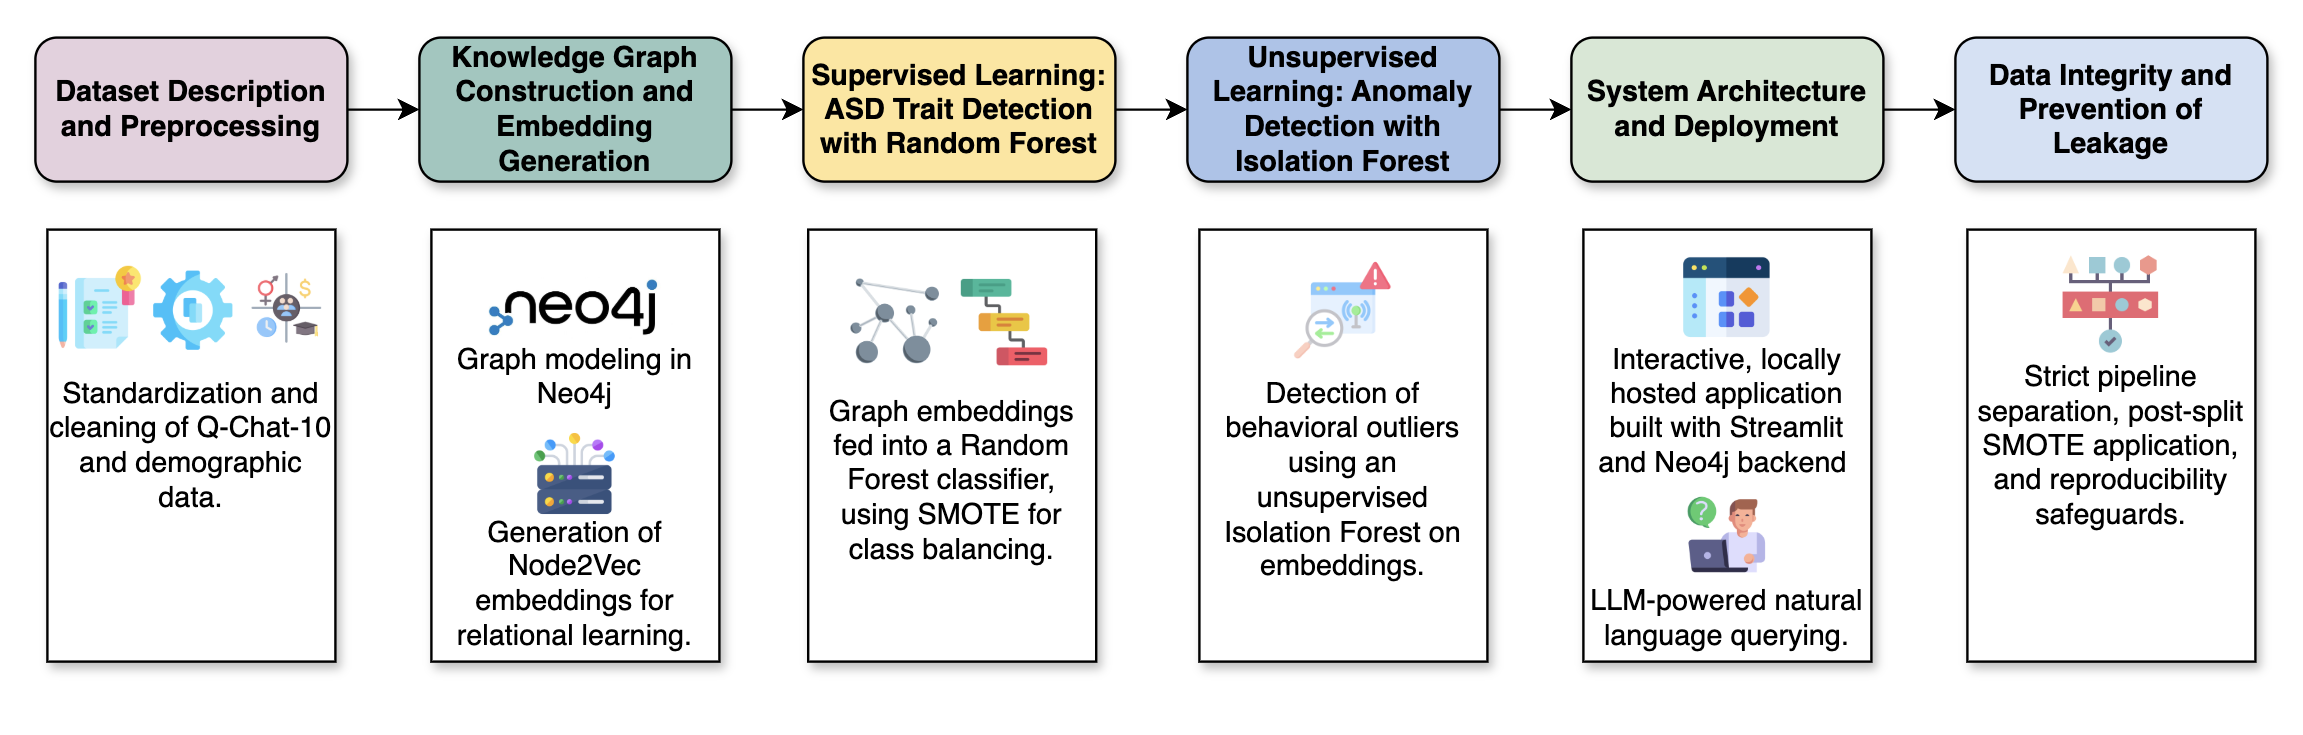
\includegraphics[width=\textwidth]{NeuroCypher Framework.png}
    \caption{Overview of the NeuroCypher Framework. Behavioral and demographic responses are transformed into a knowledge graph, encoded as embeddings, and used for downstream prediction, anomaly detection, and natural-language-driven exploration.}
    \label{fig:neurocypher-framework}
\end{figure}

\subsection{Dataset Description and Preprocessing}

This study used the \textit{Autistic Spectrum Disorder Screening Data for Toddlers}, comprising 1,054 samples and questionnaire- plus demographic-level variables. The dataset includes ten Q-Chat behavioral items (A1--A10), age in months, demographic characteristics, and the identity of the respondent. The provided target variable, \texttt{Class\_ASD\_Traits}, is generated by the screening logic of the source application. In the revised evaluation, \texttt{Qchat-10-Score} was excluded from modeling because it is directly computed from the questionnaire responses.

Preprocessing was performed with \texttt{pandas}. Numeric fields were parsed using locale-aware conversion, text fields were stripped of whitespace and normalized, and cases with missing identifiers or labels were removed. To reduce optimistic bias, duplicate rows were removed before model splitting. This step removed 79 duplicated instances from the original dataset, yielding 975 unique rows for evaluation.

\subsection{Knowledge Graph Construction and Embedding Generation}

Each preprocessed case was inserted into Neo4j as a \texttt{:Case} node. Behavioral answers were connected to \texttt{:BehaviorQuestion} nodes through \texttt{HAS\_ANSWER} relationships, demographic values were connected through \texttt{HAS\_DEMOGRAPHIC}, and respondent information through \texttt{SUBMITTED\_BY}. Additional graph variants included optional behavior-pattern, complexity, similarity, and demographic-context edges for ablation and sensitivity analysis.

Graph embeddings were generated with Node2Vec in the Python pipeline rather than through in-database graph analytics. The current implementation writes 128-dimensional embeddings back to the case nodes and uses a fixed random seed of 42 for reproducibility. To reduce transductive contamination, the revised protocol first split the deduplicated dataset into a 70/30 stratified train/test partition. The graph was then built only from the training cases. Test cases were inserted as unlabeled nodes for embedding refresh without exposing diagnostic labels during graph generation. This design does not eliminate all limitations of the underlying screening task, but it substantially reduces leakage relative to the original all-cases graph construction.

\subsection{Predictive Evaluation Design}

Three predictive settings were evaluated. First, a \textit{reference tabular baseline} used XGBoost on raw questionnaire and demographic variables (A1--A10, age in months, sex, ethnicity, jaundice history, family ASD history, and respondent type). Second, a \textit{graph-only baseline} used XGBoost on Node2Vec embeddings derived from the training graph. Third, a \textit{hybrid model} combined raw tabular variables with graph embeddings. All experiments used a deterministic 70/30 stratified split with 5-fold stratified cross-validation on the training partition only. Hyperparameters for XGBoost were selected through a small CV-guided search over depth, learning rate, number of trees, subsampling, column sampling, and regularization settings.

Evaluation metrics included ROC AUC, F1-score, precision, recall, and average precision. These metrics were computed on the untouched holdout set after all preprocessing, embedding generation, and parameter selection decisions were completed on the training partition.

\subsection{Data Integrity and Clinical Interpretation}

The revised experiments identified an important methodological issue in the source dataset: the published class label is deterministically derived from the same questionnaire responses used as predictors. From a clinical perspective, this means that very high questionnaire-based predictive scores do not necessarily indicate meaningful diagnostic intelligence; they may largely reflect recovery of the source screening rule. For this reason, the raw tabular model is retained as a strong \textit{reference baseline}, but not interpreted as evidence of independent diagnostic generalization.

Accordingly, the primary value of NeuroCypher is not framed as replacing established screening instruments through superior predictive accuracy. Rather, the framework is intended to support clinicians through structured, context-aware exploration of behavioral and demographic patterns. The knowledge graph enables case comparison, pattern inspection, anomaly flagging, and natural-language access to the data, thereby functioning as a decision-support layer around existing screening workflows.

\section{Results}\label{sec2}

The revised experiments were designed to distinguish rule-recovery performance from representation-based analysis while preserving the full NeuroCypher pipeline. After deduplication and split-first evaluation, we examined six complementary components: (i) semantic querying over the knowledge graph, (ii) a tabular XGBoost reference baseline, (iii) a graph-only embedding model, (iv) a hybrid tabular-plus-graph model, (v) graph ablations and weight-sensitivity analysis, and (vi) SHAP-based global and case-level interpretation of the graph classifier.

\subsection{Semantic Querying and Graph Exploration}

The natural-language interface remained operational in the revised pipeline and continued to provide structured access to the graph without requiring Cypher expertise. In practice, this component enables clinicians and educators to query counts, subgroups, and case patterns directly through natural language, while the underlying system translates user intent into graph queries over behavioral and demographic nodes. Although the semantic interface was not re-evaluated as a predictive module, it remains central to the framework because it exposes the graph structure in a clinically accessible form. This supports the use of NeuroCypher as an exploratory and explanatory environment rather than only as a predictive model.

\subsection{Reference Tabular, Graph-Only, and Hybrid Baselines}

Three supervised baselines were evaluated with XGBoost under a common 70/30 split and 5-fold CV protocol. The first was a reference tabular baseline using raw questionnaire and demographic variables. The second used only graph embeddings learned from the train-only knowledge graph. The third combined raw tabular variables with graph embeddings.

The tabular XGBoost reference baseline achieved very high holdout performance (ROC AUC = 0.996, F1 = 0.971, precision = 0.980, recall = 0.962, AP = 0.998). Its mean cross-validation ROC AUC on the training split was 0.997. However, because the published target label is deterministically derived from the questionnaire answers, this result should be interpreted as a strong reference baseline rather than evidence of independent diagnostic intelligence.

The hybrid raw-plus-graph model also achieved very high holdout performance (ROC AUC = 0.994, F1 = 0.962, precision = 0.949, recall = 0.976, AP = 0.998; CV ROC AUC = 0.996). This is consistent with the fact that the hybrid model inherits the highly informative questionnaire signal. By contrast, the graph-only baseline yielded substantially weaker holdout discrimination (ROC AUC = 0.485, F1 = 0.781, precision = 0.700, recall = 0.885, AP = 0.718), despite a more optimistic training CV ROC AUC of 0.739. Thus, tuning improved graph-only cross-validation behavior but did not translate into meaningful holdout generalization.

Taken together, these findings suggest that the graph representation is not, by itself, a superior predictive substitute for the raw questionnaire on this dataset. Instead, its value is better understood in terms of structure, interpretability, and support for exploratory reasoning over case relationships.

\noindent\textbf{Table 1.} Holdout and cross-validation performance for the three main supervised baselines under the leakage-safer split-first protocol.
\begin{center}
\scriptsize
\begin{tabular}{lrrrrrr}
\toprule
Model & Holdout ROC AUC & F1 & Precision & Recall & AP & CV ROC AUC \\
\midrule
Raw tabular reference & 0.996 & 0.971 & 0.980 & 0.962 & 0.998 & 0.997 \\
Raw + graph & 0.994 & 0.962 & 0.949 & 0.976 & 0.998 & 0.996 \\
Graph only & 0.486 & 0.781 & 0.700 & 0.885 & 0.718 & 0.739 \\
\bottomrule
\end{tabular}

\end{center}

\subsection{Graph Ablation Analysis}

To assess how graph design choices affected downstream separability, we evaluated several graph variants. The strongest holdout ROC AUC among the graph-based ablations was observed for the full graph pipeline and the anomaly-gated full graph pipeline (both ROC AUC = 0.568, F1 = 0.824, precision = 0.730, recall = 0.947). Removing similarity edges reduced holdout ROC AUC to 0.524 with F1 = 0.813, while the simplified graph pipeline yielded ROC AUC = 0.483 with F1 = 0.830. Removing demographic context produced the weakest holdout ROC AUC (0.440) with F1 = 0.811. 

The ablation results show that graph composition materially changes downstream behavior, but the resulting gains remain modest under stricter data separation. In particular, the graph variants preserve relatively high recall while failing to achieve strong ROC discrimination, which is consistent with a representation that captures broad structural regularities but not a stable predictive boundary on the held-out cases.

\noindent\textbf{Table 2.} Ablation analysis of graph construction choices. Coverage and rejection-rate columns are retained because the anomaly-gated setting functions as a reject-option variant rather than a standard classifier.
\begin{center}
\scriptsize
\begin{tabular}{lrrrrr}
\toprule
Graph variant & Holdout ROC AUC & F1 & Precision & Recall & AP \\
\midrule
Full graph pipeline & 0.568 & 0.824 & 0.730 & 0.947 & 0.740 \\
Full graph + anomaly gate & 0.568 & 0.824 & 0.730 & 0.947 & 0.740 \\
No similarity edges & 0.524 & 0.813 & 0.710 & 0.952 & 0.755 \\
Current graph pipeline & 0.508 & 0.780 & 0.697 & 0.885 & 0.711 \\
No behavior patterns & 0.508 & 0.780 & 0.697 & 0.885 & 0.711 \\
Simplified graph pipeline & 0.484 & 0.830 & 0.710 & 1.000 & 0.715 \\
No demographic context & 0.440 & 0.812 & 0.707 & 0.952 & 0.679 \\
\bottomrule
\end{tabular}

\end{center}

\subsection{Weight Sensitivity}

We further examined whether manually assigned edge weights materially affected graph-based performance. The best holdout configuration was a global +10\% perturbation of the heuristic weights, with ROC AUC = 0.551, F1 = 0.825, precision = 0.709, recall = 0.986, and AP = 0.738. The heuristic baseline itself achieved ROC AUC = 0.532 and F1 = 0.821, whereas the uniform-weight configuration dropped to ROC AUC = 0.457 and F1 = 0.802. Other perturbations produced ROC AUC values between 0.500 and 0.539. The sensitivity analysis was therefore labeled \textit{sensitive}, indicating that graph-based behavior depends on parameterization, even if absolute holdout discrimination remains limited.

An important observation is that several weight configurations produced high training CV ROC AUC values (approximately 0.91--0.95) while remaining close to chance on the holdout set. This divergence suggests that graph parameter tuning can easily overstate apparent performance if judged only on internal resampling, reinforcing the need for strict held-out evaluation.

\noindent\textbf{Table 3.} Sensitivity of graph-only performance to manual edge-weight configurations.
\begin{center}
\scriptsize
\begin{tabular}{lrrrrr}
\toprule
Configuration & Holdout ROC AUC & F1 & Precision & Recall & AP \\
\midrule
All weights +10\% & 0.551 & 0.825 & 0.709 & 0.986 & 0.738 \\
All weights -20\% & 0.539 & 0.759 & 0.720 & 0.803 & 0.748 \\
Heuristic baseline & 0.532 & 0.821 & 0.717 & 0.962 & 0.704 \\
All weights -10\% & 0.521 & 0.808 & 0.708 & 0.942 & 0.755 \\
Neutral similarity family & 0.518 & 0.810 & 0.710 & 0.942 & 0.714 \\
Neutral demographic risk weights & 0.517 & 0.824 & 0.724 & 0.957 & 0.734 \\
All weights +20\% & 0.500 & 0.780 & 0.720 & 0.851 & 0.695 \\
Uniform weights & 0.457 & 0.802 & 0.701 & 0.938 & 0.681 \\
\bottomrule
\end{tabular}

\end{center}

\subsection{Interpretability, SHAP Analysis, and Clinical Utility}

The leakage-safer interpretability run yielded ROC AUC = 0.512, F1 = 0.782, precision = 0.721, recall = 0.856, and average precision = 0.733 for the graph classifier on the holdout set. Although these scores do not support strong standalone prediction claims, the SHAP analysis remained useful for examining how the graph representation behaved.

At the global level, the most influential embedding dimensions were \texttt{emb\_15}, \texttt{emb\_43}, \texttt{emb\_21}, \texttt{emb\_52}, and \texttt{emb\_95}, as shown in the packaged SHAP importance table and figures. To improve interpretability, we computed approximate embedding-to-feature mappings based on correlation structure within the training data. These mappings suggested that the most influential embedding dimensions were associated primarily with Q-Chat items such as A1, A5, A6, A7, and A9, and secondarily with demographic indicators such as ethnicity and jaundice status. These associations are explicitly approximate and do not imply one-to-one semantic equivalence between embedding dimensions and clinical variables.

\noindent\textbf{Table 4.} Top global SHAP dimensions for the graph classifier, with approximate bridges back to original questionnaire and demographic variables.
\begin{center}
\scriptsize
\begin{tabular}{lll}
\toprule
Embedding dimension & Mean absolute SHAP & Approximate dominant mapped features \\
\midrule
\texttt{emb\_15} & 0.553 & A1, A5, A9 \\
\texttt{emb\_43} & 0.467 & Ethnicity, A6, A9 \\
\texttt{emb\_21} & 0.446 & A7, A5, A1 \\
\texttt{emb\_52} & 0.350 & A6, A1, A9 \\
\texttt{emb\_95} & 0.338 & A9, A1, A8 \\
\bottomrule
\end{tabular}

\end{center}

\begin{figure}[H]
    \centering
    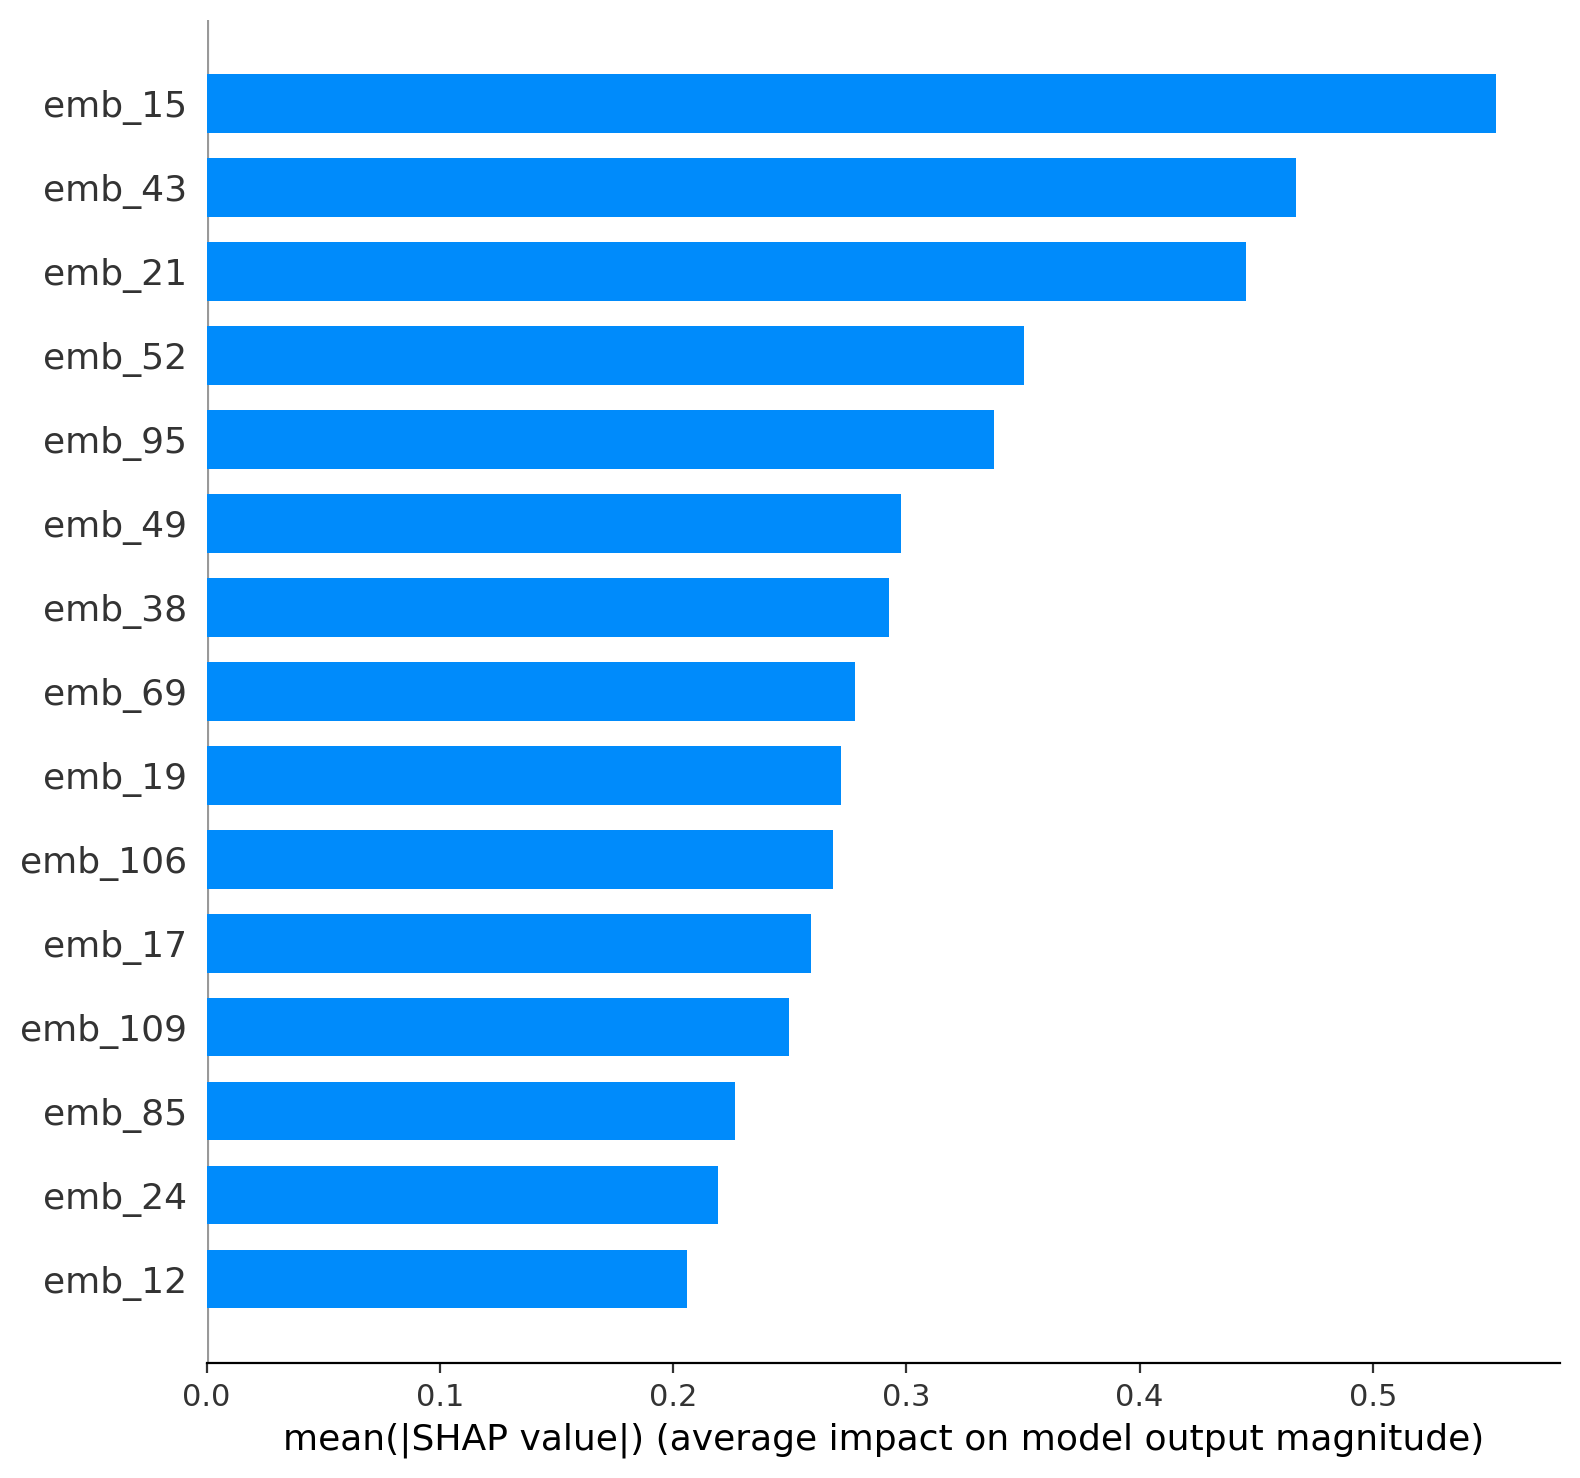
\includegraphics[width=0.92\textwidth]{figure_shap_global_bar.png}
    \caption{Global SHAP bar plot for the leakage-safer graph classifier. Larger mean absolute SHAP values indicate embedding dimensions with greater overall contribution to holdout predictions.}
    \label{fig:shap-global-bar}
\end{figure}

\begin{figure}[H]
    \centering
    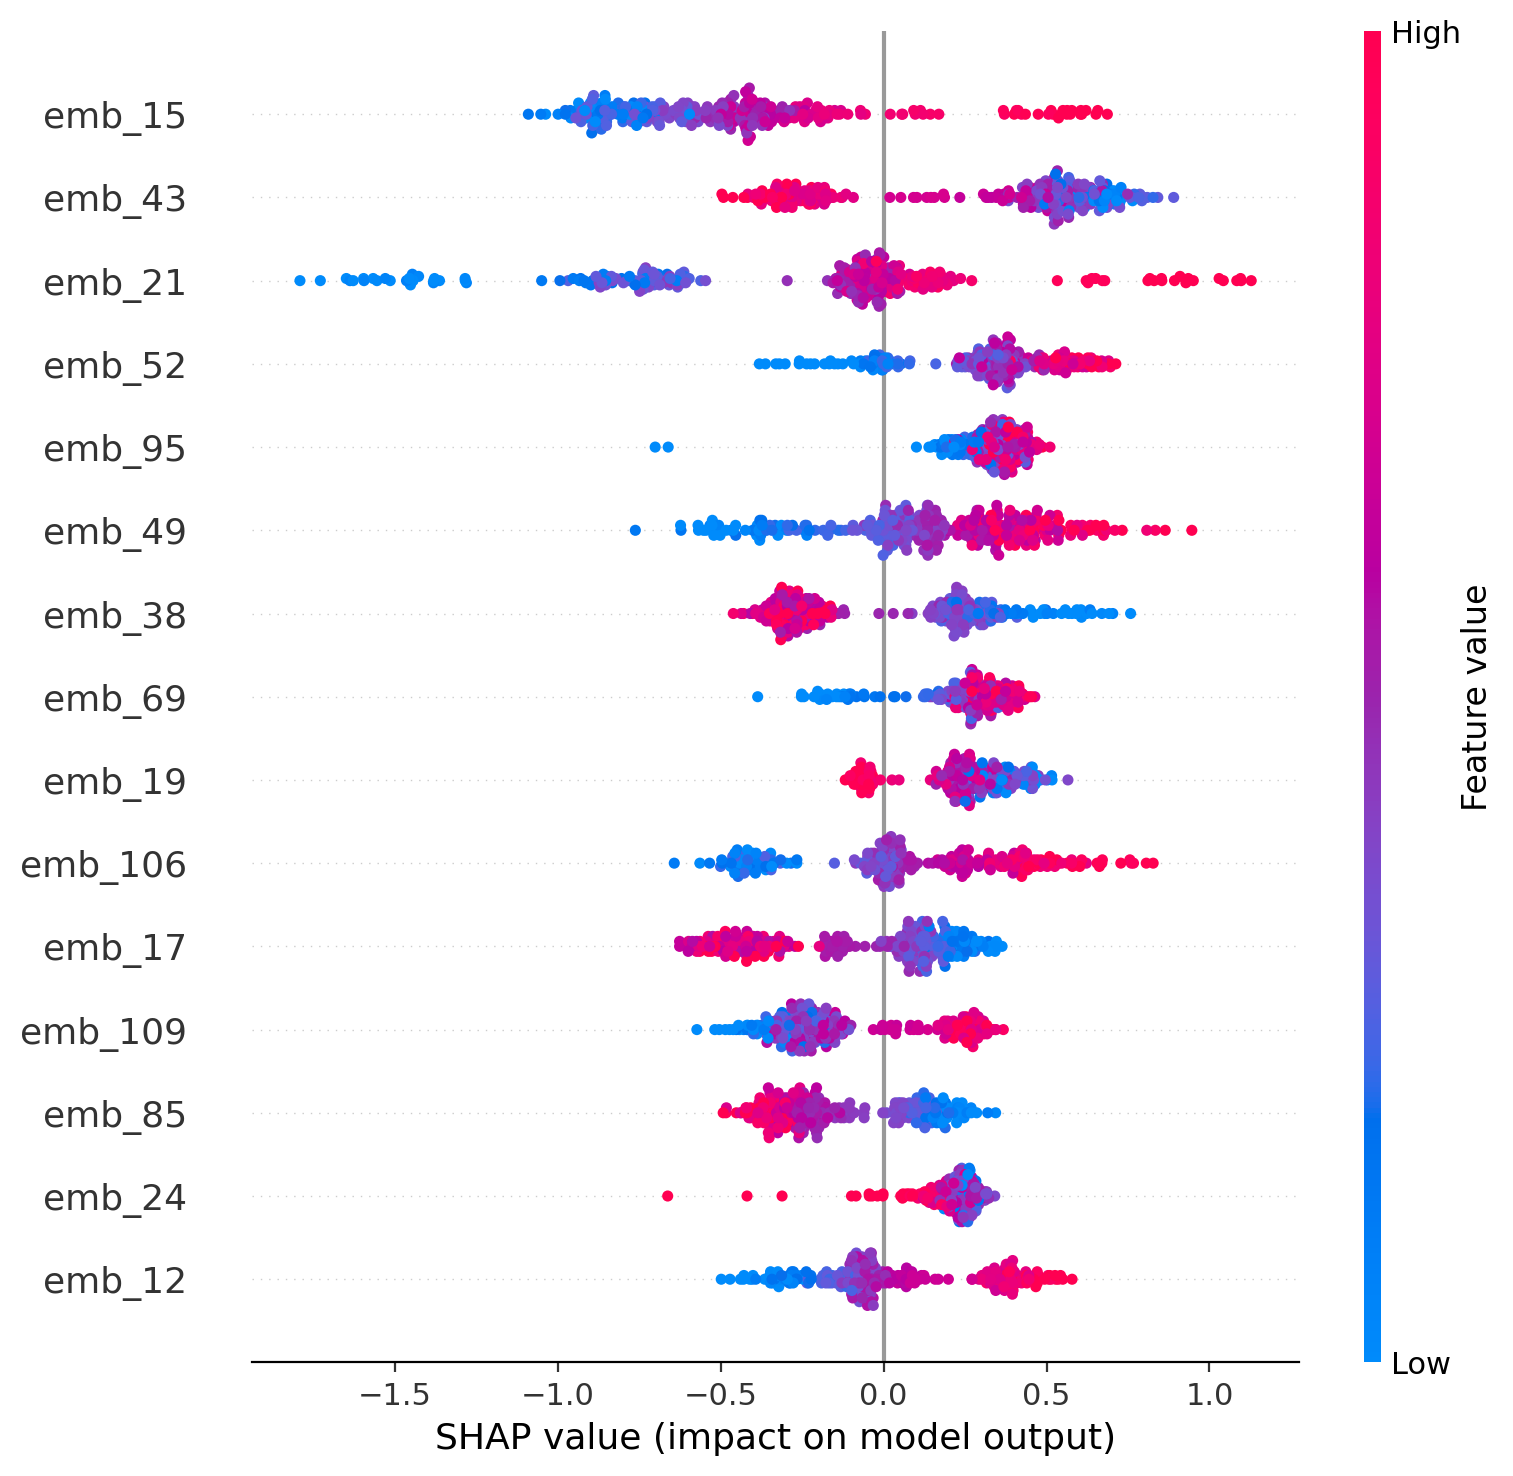
\includegraphics[width=0.92\textwidth]{figure_shap_beeswarm.png}
    \caption{SHAP beeswarm plot for the graph classifier. The distribution of point-level contributions shows that a small subset of embedding dimensions drives most case-level variation in prediction.}
    \label{fig:shap-beeswarm}
\end{figure}

At the local level, case-based SHAP explanations identified the embedding coordinates that most strongly influenced individual predictions. For example, high-confidence positive holdout cases were repeatedly driven by combinations of \texttt{emb\_49}, \texttt{emb\_43}, \texttt{emb\_15}, \texttt{emb\_95}, \texttt{emb\_52}, and \texttt{emb\_21}. These local explanations support case comparison and pattern inspection even when the graph model is not sufficiently strong to justify autonomous prediction. In this sense, the interpretability pipeline functions as a transparency layer over the graph representation.

\noindent\textbf{Table 5.} Illustrative local explanation for a high-confidence positive holdout case. The mapped original variables are approximate correlation-based bridges rather than exact semantic decompositions of the embedding space.
\begin{center}
\scriptsize
\begin{tabular}{llll}
\toprule
Case ID & Embedding dimension & SHAP value & Approximate bridge to original variables \\
\midrule
619 & \texttt{emb\_49} & 0.437 & A5, A7, A6 \\
619 & \texttt{emb\_43} & 0.434 & Ethnicity, A6 \\
619 & \texttt{emb\_15} & -0.403 & A1, A5, A9 \\
619 & \texttt{emb\_95} & 0.383 & A9, A1, A8 \\
\bottomrule
\end{tabular}

\end{center}

\subsection{Anomaly Detection and Decision Support}

The anomaly-detection module remains part of the deployed NeuroCypher pipeline and is used as a supporting mechanism for identifying atypical cases or data profiles that deviate from the learned graph-embedding distribution. In the ablation study, an anomaly-gated evaluation variant was also tested. Although this variant did not improve holdout ROC AUC beyond the full graph pipeline, it preserved the same discrimination level while offering a reject-option design for decision support. This is clinically relevant because the practical utility of anomaly detection lies less in maximizing average predictive performance and more in highlighting cases that may require closer inspection, follow-up review, or data-quality verification.

From a clinical perspective, the revised findings indicate that high predictive accuracy in questionnaire-based ASD screening should not be conflated with richer diagnostic reasoning when the target variable is constructed from the same behavioral inputs. Under this interpretation, the principal contribution of NeuroCypher lies in transforming tabular screening data into a structured and explorable graph representation that can support comparison of cases, inspection of local patterns, and transparent discussion of behavioral profiles in practice.




  \section{Discussion}\label{sec12}
  The results of this study highlight the effectiveness and practicality of combining symbolic reasoning with statistical
  learning to enable interpretable and user-friendly autism screening in everyday, non-clinical settings e.g. school-based
  environments. The integration of a KG with a LLM allowed for real-time, natural language querying of graph-structured data,
  significantly lowering the technical barrier for non-expert users such as educators and occupational therapists. This approach
  aligns with previous findings that emphasize the utility of NLP technologies in educational contexts to augment user experience
  and engagement (\cite{10.1109/access.2022.3177752, 10.1609/aaai.v30i1.9879}). By facilitating easier access to complex data
  through natural language interfaces, the framework effectively caters to the needs of practitioners who may not possess
  intensive technical expertise.

  The semantic querying interface proved effective in translating domain-relevant questions into Cypher queries and returning
  meaningful results, demonstrating the potential of LLMs to bridge user intent with formal graph-based syntax. Prior research
  supports the ability of modern NLP systems to convert complex user queries into structured formats, thereby enhancing
  interpretability (\cite{10.20944/preprints202410.1324.v1}).

  Importantly, knowledge graphs offer a more intuitive and interconnected way to organize and explore data compared to
  traditional table-based systems. While conventional databases often require intricate operations to relate distinct datasets
  (e.g., using JOINs in SQL), knowledge graphs represent entities and their relationships natively, allowing users to navigate
  and analyze data in a more holistic and exploratory manner. This structural advantage is particularly useful in autism
  screening, where uncovering patterns across interrelated behavioral indicators is essential (\cite{10.1145/3447772, 10.1109/
  access.2020.3012670}). The proposed framework enables non-expert users to engage meaningfully with complex data structures—an
  interaction that would typically demand advanced technical expertise.

  The predictive component, which leveraged graph embeddings and a Random Forest classifier, showed moderate but encouraging
  classification performance (AUC = 0.607, F1 = 0.813, Accuracy = 69.7\%). These metrics underscore the utility of using a
  relational graph structure over flat tabular data, even in relatively low-dimensional behavioral datasets. Studies have shown
  that Random Forest classifiers perform robustly in imbalanced scenarios when combined with techniques such as SMOTE
  (\cite{10.20944/preprints202410.1324.v1, 10.11591/ijece.v7i4.pp2215-2222}) in this framework, the results reinforce this
  notion, demonstrating the Random Forest's efficacy when addressing imbalanced class distributions.

  The use of SMOTE mitigated class imbalance effectively, and the F1 score suggests a high degree of balance between sensitivity
  and precision, a crucial characteristic in early ASD detection where over and under classification both carry clinical
  consequences. The positive impacts of SMOTE in boosting predictive performance have been documented extensively (\cite{10.1016/
  j.eswa.2019.113026, 10.30812/matrik.v22i2.2515})). Utilizing SMOTE not only improved predictive capability but also underscored
  the importance of exploring advanced sampling techniques to ensure the reliability of results in clinical assessments
  (\cite{10.5194/nhess-24-1913-2024}).

  Importantly, the inclusion of an unsupervised anomaly detection mechanism added an additional layer of insight. By flagging
  cases that deviate from the learned distribution of behaviors, the Isolation Forest module provides practitioners with a tool
  to detect atypical patterns that may otherwise go unnoticed. The incorporation of anomaly detection is supported by literature
  emphasizing its relevance in dynamic data environments to capture both rare and borderline cases (\cite{10.47065/
  bits.v5i1.3647, 10.26594/register.v5i2.1705}). This feature holds potential in both flagging ambiguous cases and identifying
  data entry errors or rare subtypes, thus supporting higher confidence in digital screening workflows.

  Compared to existing studies that often rely on static rule-based systems, single-modality models, or abstracted LLM
  discussions, the proposed framework provides an integrated and deployable solution. It moves beyond conceptual promise by
  offering a working proof-of-concept with natural language interaction, graph-based inference, and automated case evaluation,
  enhancing its practical application within educational and early intervention sectors. This aligns with findings that highlight
  the necessity of integrating diverse modalities in educational assessments to reap the benefits from various data sources
  (\cite{10.2991/978-94-6463-238-5_35}).

  Furthermore, it supports personalized prediction workflows, not just population-level modeling, offering value in real-world
  educational or early intervention contexts. The shift towards personalized approaches underscores a vital transition in autism
  screening methodologies that can lead to more tailored educational interventions for individuals.

  Given the increasing rates of autism diagnosis, especially in school-aged children, integrating such automated and
  interpretable screening tools into school environments could facilitate early detection and timely intervention (\cite{10.1001/
  jamanetworkopen.2022.54303, 10.4103/ijmr.ijmr_1968_16}). This is particularly critical considering that many children with
  autism may display subtle variations in behavior that traditional observation might miss. School professionals, equipped with
  these tools, can discern developmental concerns and refer children for further evaluation with greater efficiency and accuracy
  (\cite{10.3390/app6070200, 10.1001/jamapediatrics.2023.5727}).

  As an initial proof of concept, the NeuroCypher ASD framework illustrates how semantic technologies and machine learning can be
  combined into an intuitive, school-oriented tool for early autism detection. Rather than targeting clinical specialists alone,
  the system is designed to empower educational professionals to participate meaningfully in the screening process. Consider, for
  instance, a school psychologist or occupational therapist working with a small group of toddlers to identify early signs of
  autism spectrum disorder. Using NeuroCypher ASD, they can upload anonymized questionnaire data through a simple interface,
  which then processes the input, generates graph embeddings, and returns both classification results and anomaly alerts. Beyond
  static analysis, the system supports interactive exploration via natural language queries such as \textit{“Which toddlers have
  similar sensory profiles?”} or \textit{“Has this behavior pattern been linked to ASD in previous cases?”}, thus enabling a
  dynamic and interpretable workflow without requiring technical expertise. Although the tool is designed to improve
  accessibility and support early-stage identification, it is important to emphasize that it is not intended to serve as a
  standalone diagnostic instrument. The insights generated by the system should be regarded as preliminary indicators. Any
  flagged cases or risk assessments should be followed by a formal evaluation through relevant multidisciplinary committees and
  clinical experts, according to established diagnostic protocols. Furthermore, implementing such tools in educational
  environments has the potential to foster more proactive and inclusive support systems. Early identification and tailored
  interventions can contribute to improved academic and social outcomes for children with ASD, promoting long-term integration
  into mainstream educational frameworks and enhancing their overall quality of life (\cite{10.1002/aur.2033}).


  Nevertheless, certain limitations should be acknowledged. First, the relatively moderate predictive performance of the
  classifier (AUC = 0.607) suggests that more advanced classifiers or multimodal feature integration may be necessary to enhance
  robustness. This limitation is likely attributed to the nature of the dataset, which, while publicly available and valuable for
  initial prototyping, includes a relatively small number of features and lacks the depth and diversity of real-world clinical
  records. Furthermore, some questionnaire items may not possess sufficient discriminative power in isolation. Future iterations
  of the framework may benefit from feature expansion or the application of more expressive models, such as ensemble methods or
  transformer-based architectures, to improve accuracy and dependability (\cite{10.14257/astl.2016.133.15}). Second, the model
  was trained on synthetic survey data; applying the framework to real-world clinical datasets remains a key step for external
  validation. Real-world applicability is essential for confirming the practical relevance and generalizability of the model in
  school or healthcare settings (\cite{10.3390/app6070200}). Third, although interpretability is emphasized at the graph-querying
  level, model-level explainability could be further enhanced. Techniques such as SHAP values or LIME could be incorporated to
  clarify the relative importance of specific features and questionnaire responses, thereby improving transparency and fostering
  trust in practical deployment. Fourth, while Node2Vec was selected due to its efficiency and suitability for small to medium-
  scale graphs, future work may explore advanced embedding techniques such as Graph Convolutional Networks (GCN), Graph Attention
  Networks (GAT), or GraphSAGE. These methods may better capture nuanced semantic relationships between entities in the knowledge
  graph, especially as the ontology grows in size and complexity. Finally, although the natural language interface proved
  effective for simple questions, it currently struggles with complex multi-hop queries or aggregated logic (e.g., conditional
  filtering across entities). This limitation reflects broader challenges in the field, where increasing query complexity demands
  the evolution of NLP-to-graph translation architectures capable of managing layered reasoning across semantic relationships.

  This work represents the initial introduction and proof-of-concept implementation of the NeuroCypher ASD framework. Its primary
  goal is to demonstrate the feasibility of combining knowledge graphs, natural language interfaces, and machine learning to
  support interpretable autism screening in school-based environments. While the current version offers a functional prototype,
  future releases will extend its capabilities, address the identified limitations, and incorporate real-world data and feedback
  to ensure practical relevance and broader impact.



  \section{Conclusion}\label{sec13}
  This study presents NeuroCypher, a novel, interpretable framework that combines knowledge graphs, natural language processing,
  and machine learning to enable accessible, real-time screening for ASD in toddlers. Designed for nonclinical, resource-limited
  settings, such as schools, NeuroCypher addresses key barriers in early detection of ASD and serves as a supportive screening
  aid - not a diagnostic tool. By transforming structured questionnaire and demographic data into a semantically enriched
  knowledge graph, and by embedding that structure into vector space using Node2Vec, the system enables both predictive and
  exploratory analyses within a unified interface.

  The supervised learning component of NeuroCypher demonstrated promising performance, achieving an F1 score of 0.813 and an
  overall accuracy of 69.7\%, even when applied to a relatively small, imbalanced dataset. These results underscore the efficacy
  of graph-embedded learning and ensemble classification in low-dimensional behavioral health contexts. Additionally, an
  unsupervised anomaly detection module provided further decision support by flagging atypical cases that may warrant closer
  examination—enhancing the system’s sensitivity to edge cases or data irregularities.

  Perhaps most notably, the integration of a large language model allows users to interact with the system through natural
  language queries, translating plain-text questions into Cypher commands and executing them over the knowledge graph. This
  interface significantly lowers the barrier for educators, therapists, and school psychologists to engage with complex data
  structures, promoting user autonomy and interpretability.

  The system is deployed as a locally hosted, interactive application, offering case uploads, visual model diagnostics, and
  semantic querying—all without requiring internet access or programming knowledge. These design choices make NeuroCypher not
  only technically robust but also pragmatically deployable, offering a path toward democratized, school-based digital screening.

  While the current proof-of-concept demonstrates strong foundational capabilities, several limitations remain. Future work will
  focus on incorporating real-world clinical datasets, expanding the feature space with multimodal inputs (e.g., speech, video,
  or caregiver narratives), enhancing model-level explainability with techniques such as SHAP or LIME, and refining the LLM
  interface to support more complex, multi-hop queries. These improvements will further enhance NeuroCypher’s usability,
  reliability, and real-world relevance.

  In summary, NeuroCypher illustrates how combining symbolic and statistical AI within an accessible interface can bring high-
  impact, data-driven tools to early childhood intervention settings. By empowering non-technical stakeholders to explore and
  interpret ASD-related data in real time, the framework represents a meaningful step toward scalable, explainable, and inclusive
  healthcare informatics.



  \backmatter

  \bmhead{Supplementary information}

  If your article has accompanying supplementary file/s please state so here.

  Authors reporting data from electrophoretic gels and blots should supply the full unprocessed scans for key as part of their
  Supplementary information. This may be requested by the editorial team/s if it is missing.

  Please refer to Journal-level guidance for any specific requirements.

  \bmhead{Acknowledgements}

  Acknowledgements are not compulsory. Where included they should be brief. Grant or contribution numbers may be acknowledged.

  Please refer to Journal-level guidance for any specific requirements.


  \bibliography{sn-bibliography}

  \section*{Declarations}

  Some journals require declarations to be submitted in a standardised format. Please check the Instructions for Authors of the
  journal to which you are submitting to see if you need to complete this section. If yes, your manuscript must contain the
  following sections under the heading `Declarations':

  \begin{itemize}
  \item Funding
  \item Conflict of interest/Competing interests (check journal-specific guidelines for which heading to use)
  \item Ethics approval and consent to participate
  \item Consent for publication
  \item Data availability
  \item Materials availability
  \item Code availability
  \item Author contribution
  \end{itemize}

  \noindent
  If any of the sections are not relevant to your manuscript, please include the heading and write `Not applicable' for that
  section.

  %%===================================================%%
  %% For presentation purpose, we have included        %%
  %% \bigskip command. Please ignore this.             %%
  %%===================================================%%
  \bigskip
  \begin{flushleft}%
  Editorial Policies for:

  \bigskip\noindent
  Springer journals and proceedings: \url{https://www.springer.com/gp/editorial-policies}

  \bigskip\noindent
  Nature Portfolio journals: \url{https://www.nature.com/nature-research/editorial-policies}

  \bigskip\noindent
  \textit{Scientific Reports}: \url{https://www.nature.com/srep/journal-policies/editorial-policies}

  \bigskip\noindent
  BMC journals: \url{https://www.biomedcentral.com/getpublished/editorial-policies}
  \end{flushleft}

  \begin{appendices}

  \section{Section title of first appendix}\label{secA1}

  An appendix contains supplementary information that is not an essential part of the text itself but which may be helpful in
  providing a more comprehensive understanding of the research problem or it is information that is too cumbersome to be included
  in the body of the paper.

  %%=============================================%%
  %% For submissions to Nature Portfolio Journals %%
  %% please use the heading ``Extended Data''.   %%
  %%=============================================%%

  %%=============================================================%%
  %% Sample for another appendix section			       %%
  %%=============================================================%%

  %% \section{Example of another appendix section}\label{secA2}%
  %% Appendices may be used for helpful, supporting or essential material that would otherwise
  %% clutter, break up or be distracting to the text. Appendices can consist of sections, figures,
  %% tables and equations etc.



  \end{appendices}

  %%===========================================================================================%%
  %% If you are submitting to one of the Nature Portfolio journals, using the eJP submission   %%
  %% system, please include the references within the manuscript file itself. You may do this  %%
  %% by copying the reference list from your .bbl file, paste it into the main manuscript .tex %%
  %% file, and delete the associated \verb+\bibliography+ commands.                            %%
  %%===========================================================================================%%




  \end{document}
